% Notation des isotopes
% Usage :
%	\noyau{X}{A}{Z}
\newcommand{\noyau}[3]{ % package mathtools
	{\prescript{#2}{#3}{\ch{#1}}}
}

% On utilisera plutôt la commande \isotope du module chemmacros :
%	\isotope{C} <-> \noyau{C}{12}{6}
%	\isotope*{C} <-> \noyau{C}{12}{}
%	\isotope{14,C} <-> \noyau{C}{14}{6}
%	\isotope*{14,C} <-> \noyau{C}{14}{}



% Dessiner un petit noyau avec tikz
% Le paramètre permet de modifier la graine du générateur aléatoire
% pour dessiner des noyaux différents
\newcommand\smallnucleus[1][1]{
	\begin{tikzpicture}
		\pgfmathdeclarerandomlist{color}{{red}{white}}
		\pgfmathsetseed{#1}
		\foreach \A/\R in {8/0.32,5/0.18,1/0}{
		      \pgfmathsetmacro{\S}{360/\A}
	           \foreach \B in {0,\S,...,360}{
	               \pgfmathrandomitem{\C}{color}
	               \shade[ball color=\C] (\B+\A:\R) circle (5pt);
	           }
		}
	\end{tikzpicture}
}


% Dessiner un noyau de taille moyenne avec tikz
% Le paramètre permet de modifier la graine du générateur aléatoire
% pour dessiner des noyaux différents
\newcommand\nucleus[1][1]{
	\begin{tikzpicture}
		\pgfmathdeclarerandomlist{color}{{red}{white}}
		\pgfmathsetseed{#1}
		\foreach \A/\R in {12/0.42,7/0.3,1/0}{
		      \pgfmathsetmacro{\S}{360/\A}
	           \foreach \B in {0,\S,...,360}{
	               \pgfmathrandomitem{\C}{color}
	               \shade[ball color=\C] (\B+\A:\R) circle (5pt);
	           }
		}
	\end{tikzpicture}
}

% Dessiner un gros noyau avec tikz
% Le paramètre permet de modifier la graine du générateur aléatoire
% pour dessiner des noyaux différents
\newcommand\bignucleus[1][1]{
	\begin{tikzpicture}
		\pgfmathdeclarerandomlist{color}{{red}{white}}
		\pgfmathsetseed{#1}
		\foreach \A/\R in {20/0.62,12/0.5,7/0.3,1/0}{
		      \pgfmathsetmacro{\S}{360/\A}
	           \foreach \B in {0,\S,...,360}{
	               \pgfmathrandomitem{\C}{color}
	               \shade[ball color=\C] (\B+\A:\R) circle (5pt);
	           }
		}
	\end{tikzpicture}
}

% Dessiner un proton avec tikz
\newcommand\proton{
	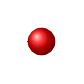
\begin{tikzpicture}
		\shade[ball color=red] (0,0) circle (5pt);
	\end{tikzpicture}
}

% Dessiner un neutron avec tikz
\newcommand\neutron{
	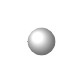
\begin{tikzpicture}
		\shade[ball color=white] (0,0) circle (5pt);
	\end{tikzpicture}
}